\section{performance evaluation}
\label{sec:performance evaluation}
We first describe the simulation setup, then present the simulation results.
\subsection{Simulation setup}
We use the topology trace published by Huawei to evaluate the performance of our proposed scheme (named by \CI). As introduced in related work, unavoidable traps are caused by the topology constraints. The topology trace provided by Huawei does not have unavoidable traps. That is,  although a BP path may not be able to be found for an AP path, there does exist two SRLG-disjoint paths in the network between the source node to the destination node. As the topology trace has 17 different topologies with various number of nodes, links, and link weights, we compare our algorithm with other peer algorithms using each topology. Table \ref{tab:AllSample} shows the basic network setting in these 17 topologies. After normalizing the result in each topology, we take the average of the normalized results as the final simulation result.

%\begin{table}
%  \centering
%  \begin{tabular}{*{7}{c}}
%\toprule
%Topology & 1 & 2 & 3 & 4 & 5 & 6 \\
%\midrule
%Node  & 424  & 1825 & 514&514 &8301 &1814   \\
%Edge & 1378  & 24837 & 2024& 2074& 40326&24816  \\
%\bottomrule
%\toprule
%Topology & 7&8&9&10&11&12 \\
%\midrule
%Node  &2014 & 2014&2014 & 2014& 2013&20 \\
%Edge &2068 &2068 & 2068& 2068& 15661 & 31\\
%\bottomrule
%\toprule
%Topology  &13&14&15&16&17 \\
%\midrule
%Node  &2014 &2014 & 424&2014 & 2014 & \\
%Edge & 2068& 2068&1378 & 2068&2068& \\
%\bottomrule
%\end{tabular}
%\caption{node number and edge number of 17 different topologies.}
%\label{tab:AllSample}
%\end{table}
%
\begin{table*}[tp]
\small{
  \centering
  \begin{tabular}{*{18}{c}}
\toprule
Topology & 1 & 2 & 3 & 4 & 5 & 6& 7&8&9&10&11&12&13&14&15&16&17 \\
\midrule
Node  & 424  & 1825 & 514&514 &8301 &1814 &2014 & 2014&2014 & 2014& 2013&20 &2014 &2014 & 424&2014 & 2014   \\
Edge & 1378  & 24837 & 2024& 2074& 40326&24816 &2068 &2068 & 2068& 2068& 15661 & 31& 2068& 2068&1378 & 2068&2068 \\
\bottomrule
\end{tabular}
}
\caption{node number and edge number of 17 different topologies.}
\label{tab:AllSample}
\end{table*}
For performance comparisons, besides our scheme (named by \CI), we also implemented other four SRLG-disjoint routing algorithms as follows:


\begin{enumerate}
  \item ILP: The work in~\cite{hu2003diverse}  aims to find SRLG-disjoint paths through an ILP formulation such that the total weight of the two paths are minimized. We are not aware that other studies look for the Min-Min SRLG-disjoint paths through ILP formulation. Therefore, following \cite{hu2003diverse}, we formulate  our Min-Min SRLG-disjoint routing problem by changing the objective function.
  \item IQCP: As any $0-1$ integer linear program where all variables are either 0 or 1,  ILP can be formulated as a quadratically constrained program. Different from ILP, we also model Min-Min SRLG-disjoint routing problem through the Integer Quadratic Constraints Program (IQCP)\cite{hu2003diverse}.
  \item KSP\cite{eppstein1998finding}: It finds the first $K$ shortest paths between the source and the destination as candidate APs, and then tests them one by one in the increasing order of their costs to see if it has a corresponding (disjoint) BP, until such a BP is found.
  \item CoSE\cite{rostami2007cose}: When an AP encounters a trap problem, CoSE tries a simple and exhaustive search to find a SRLG set that no AP going through the SRLG set can find the SRLG BP path. Based on the SRLG set,   it partitions the original problem based on the set and designs an algorithm to search for the SRLG disjoint path pair.
\end{enumerate}

The first two (ILP and IQCP) are based on integer program models. In our implementation, the tool GUROBI 7.0\cite{optimization2012gurobi} is employed to resolve these two integer problems. Four performance metrics are applied to evaluate the performance of different SRLG-disjoint routing algorithms:
\begin{itemize}
  \item \textbf{Path weight}: is the sum of the link weight in the path. \note{What is the weight in the evaluation?}
  \item \textbf{Path hop}: the number of hops in the path
  \item \textbf{Runtime}: the average number of milliseconds taken for SRLG-disjoint path finding.
  \item \textbf{Algorithm speedup}: Given the computation time under two different  algorithms ($alg_1$ and $alg_2$), denoted as $T_1$ and $T_2$, the algorithm speedup in the computation time of the $alg_2$ with respect to the $alg_1$: ${S_{1 - 2}} = T_1/T_2$.
  \item \textbf{Core speedup}: The core speedup \cite{bryant2003computer} of a parallel program is typically defined as
\begin{equation}
\label{equ:speed}
S_P=\frac{T_1}{T_p},
\end{equation}
where $p$ is the number of processor cores \rev{and $T_1$ and $T_p$} denote the running time on 1 core and $p$ cores, respectively.

  \item \textbf{Efficiency}: is defined \cite{bryant2003computer} as
\begin{equation}\label{equ:efficient}
E_p=\frac{S_p}{p}=\frac{T_1}{pT_p}
\end{equation}
and is typically reported as a percentage in the range (0, 1].

\end{itemize}

All simulations are run on a common PC, which is equipped with one Intel (R)  i5-5200U CPU(2.20GHz) (4 Cores) and 8.00GB RAM. To measure the computation time, we insert a timer to all the implemented algorithms.

\subsection{Performance comparison}

\subsubsection{Path Weight}
Fig.\ref{fig:normalization weitgh sum} shows the weight of AP, BP, and the sum of both AP and BP. Obviously, all implemented algorithms \CI, CoSE, KSP, ILP and IQCP achieve the same AP weight, but different BP weights thus different sum weights of AP and BP. As all the algorithms solve the same Min-Min SRLG-disjoint routing program, although they find different SRLG-disjoint path pairs, they can all achieve the goal of finding the  AP with the same least weight.
As \CI, CoSE, KSP find the  BP based on a shortest path algorithm (such as Dijkstra), they also find the BP path with the same weight. However, the two ILP-based algorithms, ILP and IQCP, focus on minimizing the weight of AP but find any BP that is SRLG-disjoint with AP, the BP paths searched by these two algorithms are different.

%\begin{figure*}[h]
%\begin{center}
%  % Requires \usepackage{graphicx}
%  \includegraphics[width=.25\textwidth]{franz/weight.eps}
%  \caption{Path weight}\label{fig:normalization weitgh sum}
%  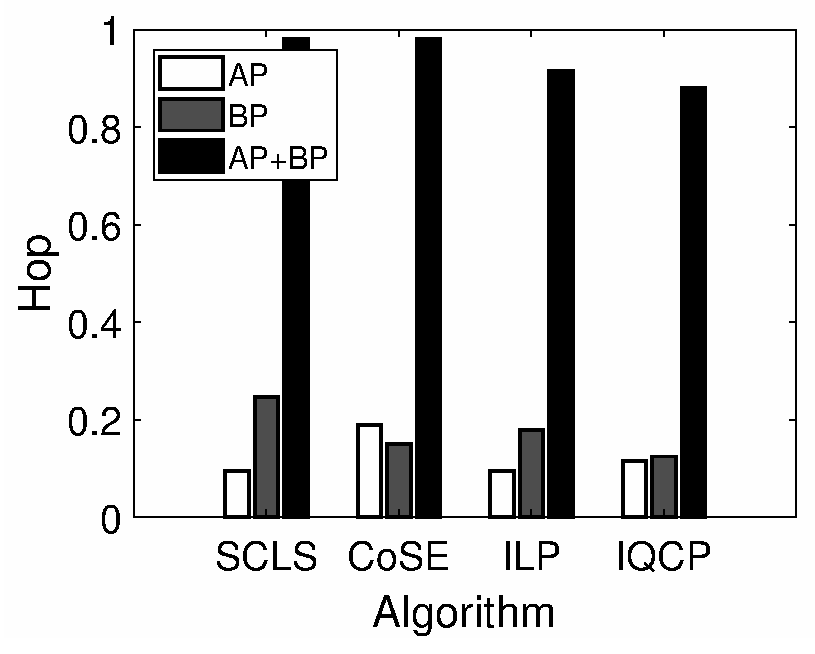
\includegraphics[width=.25\textwidth]{franz/hop.eps}
%  \caption{Path hop}\label{fig:normalization hop}
%\end{center}
% \includegraphics[width=.25\textwidth]{franz/runtime}\\
%  \caption{Runtime}\label{fig:normalization runtime}
%\end{figure*}

\begin{figure*}[tp]
\centering
\begin{minipage}[t]{0.3\linewidth}
\centering
\includegraphics[width=2.25in]{franz/weight}
\caption{Path weight}
\label{fig:normalization weitgh sum}
\end{minipage}
\hfill
\begin{minipage}[t]{0.3\linewidth}
\centering
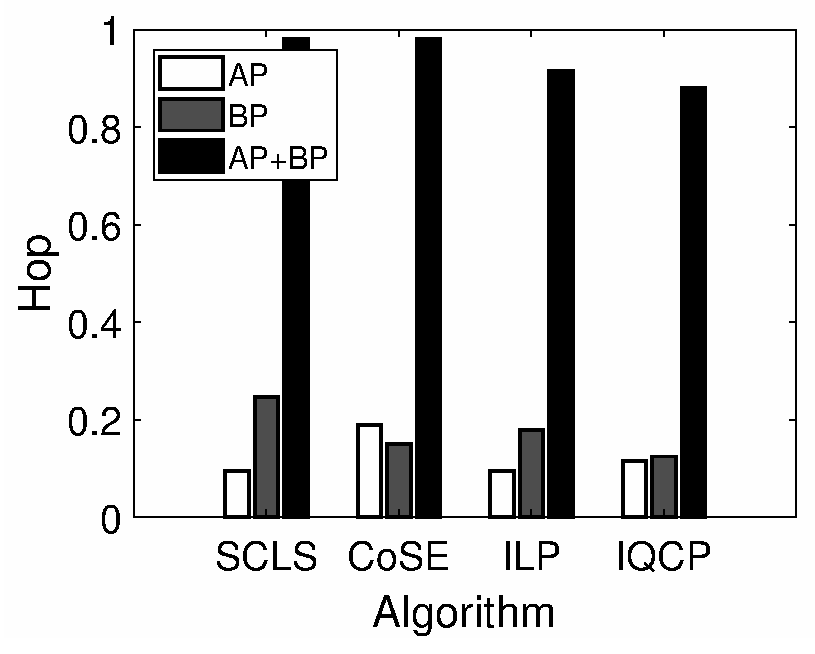
\includegraphics[width=2.25in]{franz/hop}
\caption{Path hop}
\label{fig:normalization hop}
\end{minipage}
\hfill
\begin{minipage}[t]{0.3\linewidth}
\centering
\includegraphics[width=2.25in]{franz/runtime}
\caption{Runtime}
\label{fig:normalization runtime}
\end{minipage}
\end{figure*}


\begin{figure*}[tp]
\centering
\begin{minipage}[t]{0.3\linewidth}
\centering
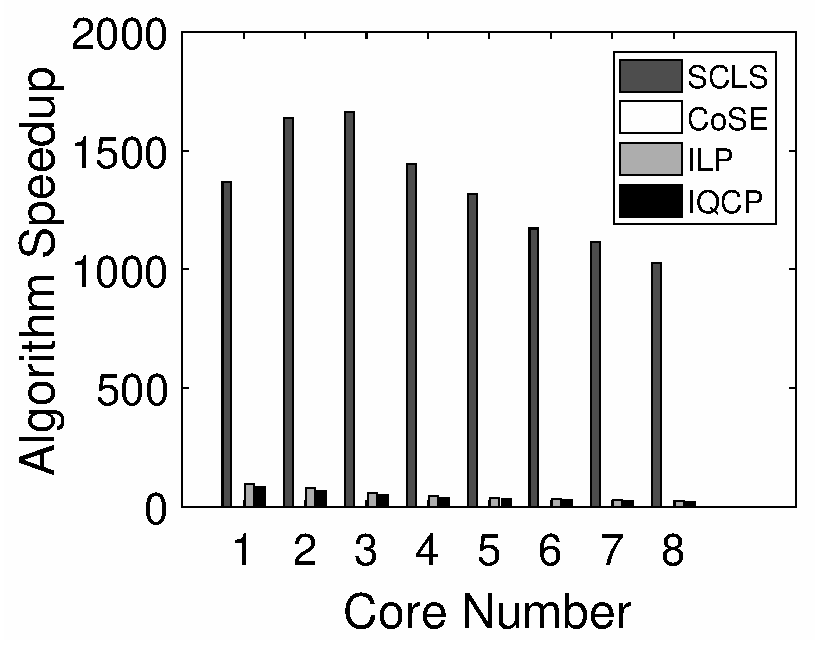
\includegraphics[width=2.25in]{franz/Multiple}
\caption{Algorithm speedup}
\label{fig:Multiple}
\end{minipage}
\hfill
\begin{minipage}[t]{0.3\linewidth}
\centering
\includegraphics[width=2.25in]{franz/speedup}
\caption{Core speedup}
\label{fig:Speedup}
\end{minipage}
\hfill
\begin{minipage}[t]{0.3\linewidth}
\centering
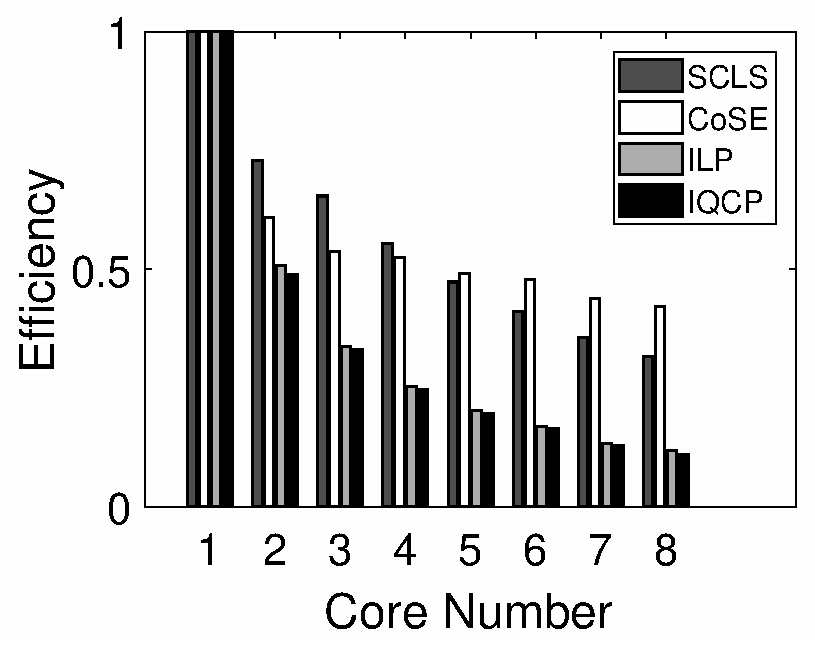
\includegraphics[width=2.25in]{franz/Efficiency}
\caption{Efficiency}
\label{fig:Efficiency}
\end{minipage}
\end{figure*}

%
%\begin{figure*}[htbp]
%\begin{minipage}[t]{0.35\linewidth}
%\centering
%\includegraphics[height=4.5cm,width=7.5cm]{franz/runtime.eps}
%\caption{one}
%\end{minipage}%
%\hfill
%\begin{minipage}[t]{0.5\linewidth}
%\centering
%\includegraphics[height=4.5cm,width=7.5cm]{franz/runtime.eps}
%\caption{two}
%\end{minipage}
%\end{figure*}

\subsubsection{Path Hop}
Fig.\ref{fig:normalization hop} shows the path hop of AP, BP, and the sum of both AP and BP. As all algorithms target to minimize the least path weight of the SRLG-disjoint path pair instead of the number of path hops, they have the same AP weight (Fig.\ref{fig:normalization weitgh sum}) even though they have different AP path hops (Fig.\ref{fig:normalization hop}). Although the AP weights under all algorithms are smaller than the BP weights in Fig.\ref{fig:normalization weitgh sum}, in Fig.\ref{fig:normalization hop}, the AP hops may not always be fewer than the BP hops.

%\begin{figure}
%  \centering
%  % Requires \usepackage{graphicx}
%  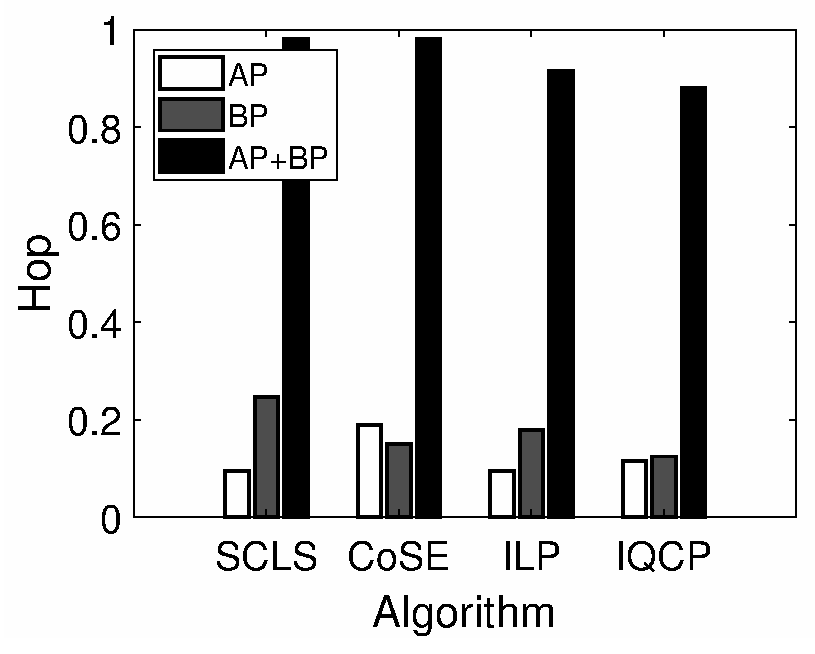
\includegraphics[width=2.35in]{franz/hop}\\
%  \caption{Path hop}\label{fig:normalization hop}
%\end{figure}

\subsubsection{Runtime}
\label{subsubsec:Runtime}
Fig.\ref{fig:normalization runtime} shows the run time under different algorithms by varying the number of CPU cores utilized.
As KSP, ILP, and IQCP are not parallel algorithms, the runtime of these algorithms under different number of cores is approximately equal. The runtime of our SCLS  and CoSE decreases with the increase of the number of processor cores because these two algorithms can partition the original problem into multiple sub-problems to execute in parallel and take advantage of the parallelism of the multi-core CPU to speed up the path searching process. Although CoSE is a parallel algorithm, the computation time is even larger than  ILP and IQCP. Some possible reasons include 1) the search process to find the conflicting SRLG set in CoSE  is not efficient; 2) As one SRLG usually includes multiple links, the partitioning of problem based on conflicting SRLG will introduce a large number of sub-problems to solve, which also results in a large computation cost.

%\begin{figure}
%  \centering
%  % Requires \usepackage{graphicx}
%  \includegraphics[width=2.35in]{franz/runtime}\\
%  \caption{Runtime}\label{fig:normalization runtime}
%\end{figure}

Different from CoSE, our SCLS looks for the set of conflicting links on an AP caught into the trap problem based on the min-cut theory in graph, and achieves the lowest time in Fig.\ref{fig:normalization runtime}. This demonstrates that our conflicting link set finding algorithm is efficient, and moreover our divide-and-conquer algorithm and intelligent AP searching process based on SRLG Conflicting Link Set can largely reduce the computation cost.

KSP is known as an effective algorithm to handle the trap problem. However, among all the algorithms implemented, the running time under KSP is the largest. A major problem of KSP is that after the current candidate AP fails the test (that is, it does not have a corresponding disjoint BP), the next candidate AP to be tested is selected solely based on the path length. In the 17 topologies we studied in the trace,  usually a large number of paths need to be tested in order to find a disjoint path pair (if it exists between a pair of nodes), thus KSP needs a large computation time.

Fig.\ref{fig:KSPproblem}  shows an example to illustrate why the KSP is extremely inefficient. In this graph, suppose SRLG conflicting link set is ${e_1,e_2}$, and the link weights of $e_1, e_2, e_3, e_4$ are much larger than other links. Then the first $K$ shortest weight paths from $s$ to $d$ will contain the shortest path segment $e_1,e_2$ denoted by the dotted line, which will further make the first shortest APs encounter the trap problem. To avoid the trap problem, $K$ have to be set as a large value, which brings a high time complexity to KSP. Different from KSP, when the shortest AP encounters the trap problem, we can quickly identify that \revtao{$\{e_1,e_2\}$} forms the SRLG conflicting link set, and then partition the original problem further into two subproblems $\mathcal{P}(\emptyset,\{e_1\})$ and \revtao{$\mathcal{P}(\{e_1\},\{e_2\})$} to execute in parallel on the multi-core CPU platform to quickly search for the SRLG disjoint path pair.

\begin{figure}[tp]
\centering
% Requires \usepackage{graphicx}
\includegraphics[width=3in]{franz/KSPproblem}
  \caption{An example to illustrate the inefficiency of KSP}
  \label{fig:KSPproblem}
\end{figure}

\subsubsection{Algorithm speedup}

In Fig.\ref{fig:Multiple}, we further compare their computation speeds. Specially, to calculate the speedup metric,
we use KSP as the baseline algorithm and set alg1 =KSP. Similar to the results in the Fig.\ref{fig:normalization runtime}, our SCLS achieves significantly larger speedup.

\subsubsection{Core speedup}

For the two parallel algorithms SCLS and CoSE, the core speedup   increases with the increase of the number of cores. %\del{Therefore, larger number of cores brings larger performance gain for these two parallel algorithms SCLS and CoSE.}
However, the increasing speed becomes smaller when the number of cores becomes larger and it incurs a higher cost to coordinate the process. Core speedup under algorithms KSP, ILP and IQCP is  approximately equal to 1 under any core number because they are not parallel algorithms. Among all algorithms, the core speedup of our SCLS is the largest, which demonstrates that our divide and conquer algorithm designed  based on the SRLG conflicting link set can bring the largest parallelism gain.

\note{How many paths pairs to search in your simulations. If you only search for one pair, then the sub=-problems may be lower than the number of cores, so multi core cannot be used.}
\subsubsection{Efficiency}
Efficiency is a measure of the overhead due to the parallelization. Programs with a high efficiency spend more time on useful work and less time on synchronization and communications. Similar to Fig.\ref{fig:Speedup}, with more cores involved, the efficiency value decreases  as a large core number brings more cost to coordinate the process. In Fig.\ref{fig:Efficiency}, the efficiency values of all algorithms decrease with the increase of the core number. Among all algorithms, the efficiency value of our SCLS is the largest under different core numbers, which demonstrates that our divide and conquer algorithm designed  based on the SRLG conflicting link set can bring the largest parallelism gain.



%\begin{figure}
%  \centering
%  % Requires \usepackage{graphicx}
%  \includegraphics[width=2.35in]{franz/runtime_nocose}\\
%  \caption{Normalization Runtime without CoSE value}\label{fig:normalization runtime_nocose}
%\end{figure}
%\subsubsection{Runtime's variance}
% As shown in Fig.\ref{fig:normalization runtime_var}.
%\begin{figure}
%  \centering
%  % Requires \usepackage{graphicx}
%  \includegraphics[width=2.35in]{franz/runtime_var}\\
%  \caption{Normalization Runtime Variance}\label{fig:normalization runtime_var}
%\end{figure}

%\subsubsection{Speed}
%The speedupSCLSte{bryant2003computer} of a parallel program is typically defined as
% \begin{equation}\label{equ:speed}
%   S_P=\frac{T_1}{T_p}
%\end{equation}
%where p is the number of processor cores and $T_k$ is the running time on k cores.Calculating the speedup of every processor cores in all algorithms in Fig.\ref{fig:Speedup} by the runtime of all algorithm from Fig.\ref{fig:normalization runtime}. The speedup value of CoSE increase with increasing the number of processor cores. The speedup value of CSLIE firstly increase then decrease because four cores is neck bottle of parallelism for CSLIE heuristic in this samples. The speedup value of other algorithm is affected slightly by the number of core processors.
%\begin{figure}
%  \centering
%  % Requires \usepackage{graphicx}
%  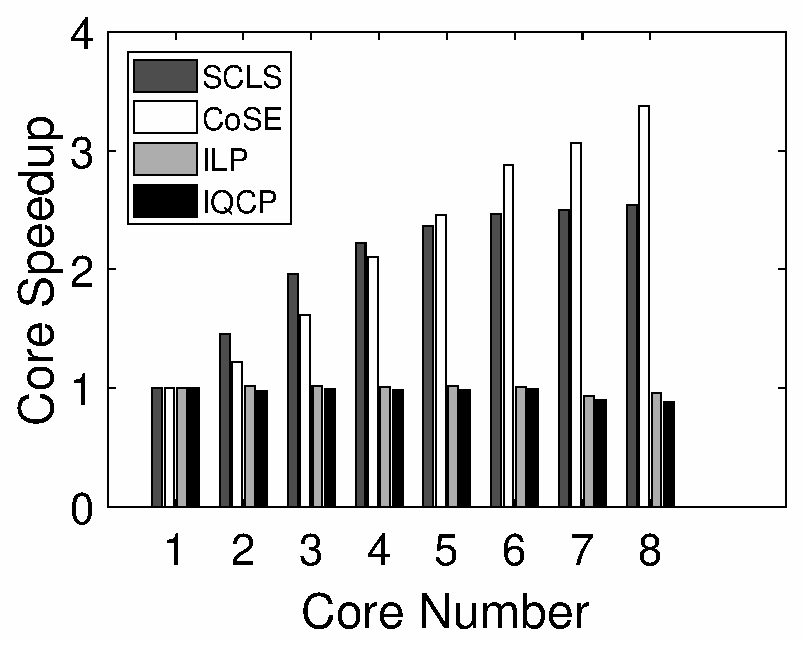
\includegraphics[width=2.35in]{franz/Speedup}\\
%  \caption{Speedup}\label{fig:Speedup}
%\end{figure}
%
%
%\subsubsection{Efficient}
%A related measureSCLSte{bryant2003computer} in Fig.\ref{fig:Efficiency}, known as efficiency, is defined as
%\begin{equation}\label{equ:efficient}
%  E_p=\frac{S_p}{p}=\frac{T_1}{pT_p}
%\end{equation}
%and is typically reported as a percentage in the range (0, 100]. Efficiency is a measure of the overhead due to parallelization. Programs with high efficiency are spending more time doing useful work and less time synchronizing and communicating than programs with low efficiency. Efficiet value of all algorithm decrease with the increase of core processors.
%\begin{figure}
%  \centering
%  % Requires \usepackage{graphicx}
%  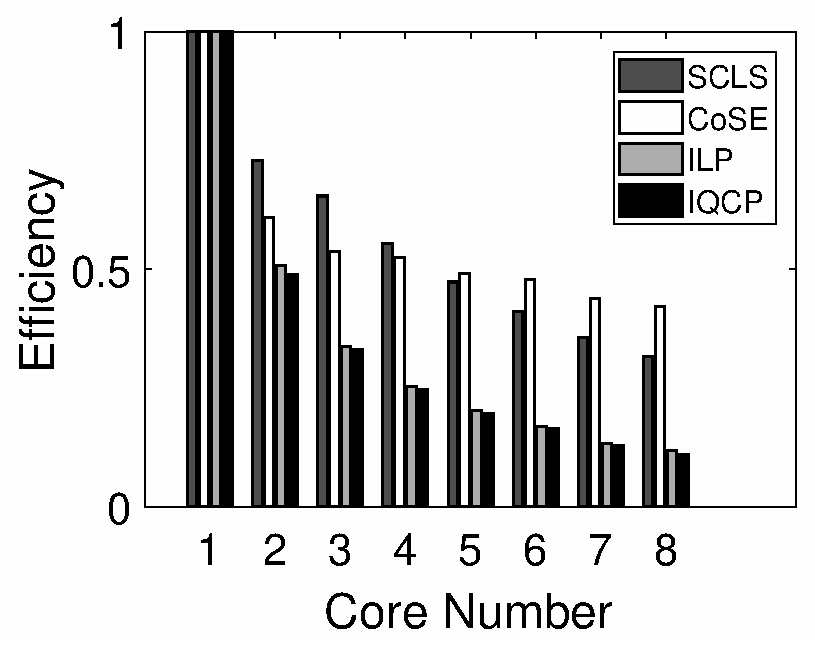
\includegraphics[width=2.35in]{franz/Efficiency}\\
%  \caption{Efficiency}\label{fig:Efficiency}
%\end{figure}
%\subsubsection{Multiple}
%The multiple's definition of parallel typically defined as
%\begin{equation}\label{equ:multiple}
%  M_n^x=\frac{T_n^{ILP}}{T_n^x}
%\end{equation}
%where x is algorithm such as CSLIE,CoSE,KSP ILP and IQCP. $T_n^x$ is the runtime of x algorithm in n processor cores. $T_n^{ILP}$ is the runtime of ILP in n processor cores. All algorithm compares with ILP runtime in Fig.\ref{fig:Multiple}
